\section{INTEGER ORDER METHODS}
\begin{frame}{INTEGER ORDER METHODS}
    The following initial value problem (IVP) will be treated:
    \begin{equation}
        \begin{cases}
        y'=f\left(t,y\right)&
        \\y(0)=y_0\,,\quad t\in[0,T]&
        \end{cases}
    \end{equation}
    \begin{multicols}{2}
    Example:
    \begin{equation}\label{eq:pvi_ex1}
        \begin{cases}
            y'-y=0&\\
            y(0)=-3&
        \end{cases}
    \end{equation}
    The exact solution to this problem is given by
    \begin{equation}
        y(t)=-3e^{-t}
    \end{equation}
    
    \columnbreak
    \begin{figure}[H]
        \centering
        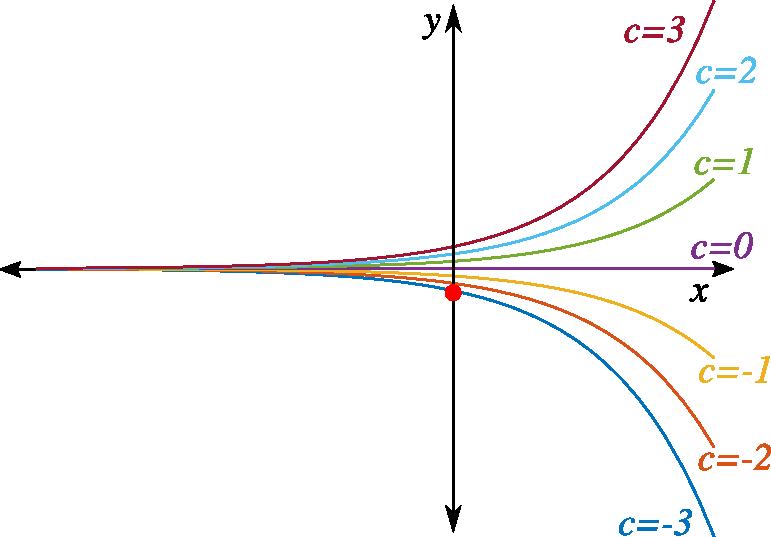
\includegraphics[scale=0.4]{files/ex_ivp_1.pdf}
        \caption{Solution for problem \ref{eq:pvi_ex1}.}
    \end{figure}
    \end{multicols}
\end{frame}



\subsection{Fourth-Order Runge-Kutta Method (RK4)}
\begin{frame}{INTEGER ORDER METHODS}
    \framesubtitle{Fourth-Order Runge-Kutta Method (RK4)}
    \begin{itemize}
        \item Improved Euler with more accuracy.
        \item $4^{th} order$ $\rightarrow$ optimal.
    \end{itemize}
    This method approximates the solution to the IVP as follows:
    
    \begin{equation}
        \begin{split}
            y_{i+1}=y_i+h\left(\dfrac{k_1+2k_2+2k_3+k_4}{6}\right)
        \end{split}
    \end{equation}
    where
    \begin{multicols}{2}
    \begin{equation*}
    \begin{array} { l } { k _ { 1 } = f \left( t _ { i } , y _ { i } \right) } \\
    { k _ { 2 } = f \left( t _ { i } + h / 2 , y _ { i } + h k _ { 1 } / 2 \right) } \\
    { k _ { 3 } = f \left( t _ { i } + h / 2 , y _ { i } + h k _ { 2 } / 2 \right) } \\ 
    { k _ { 4 } = f \left( t _ { i } + h , y _ { i } + h k _ { 3 } \right) } \end{array}
\end{equation*}
The algorithm works as
\begin{center}
    \texttt{y = runge\_kutta(f,y0,T,N)}
\end{center}
\columnbreak
\begin{figure}[H]
    \centering
    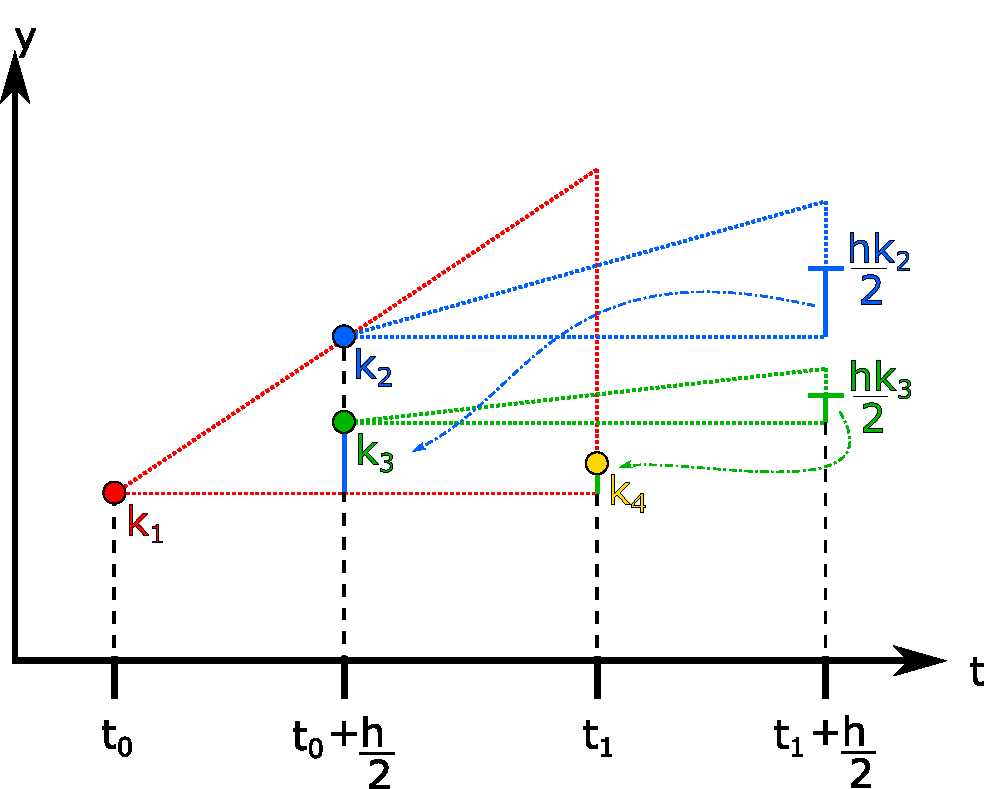
\includegraphics[scale=0.275]{files/sv.pdf}
\end{figure}
\end{multicols}


\end{frame}

\subsection{Comparison Euler - RK4}
\begin{frame}{INTEGER ORDER METHODS}
    \framesubtitle{Comparison Euler - RK4}
    \textbf{Example: approximate a solution to the IVP} 
    \begin{equation}
    \begin{cases}
        y' = 10e^{-\frac{(t-2)^2}{2}}\left(10\cos(10t)-(t-2)\sin(10t)\right)&\\ 
        y(0) = 0&
    \end{cases}
    \end{equation}
The exact solution to this problem is
\begin{equation}
    y(t) = 10e^{-\frac{(t-2)^2}{2}}\sin(10t)
\end{equation}
\begin{multicols}{2}
$\qquad\quad$\textbf{Euler}\begin{figure}[H]
        \centering
        \only<1>{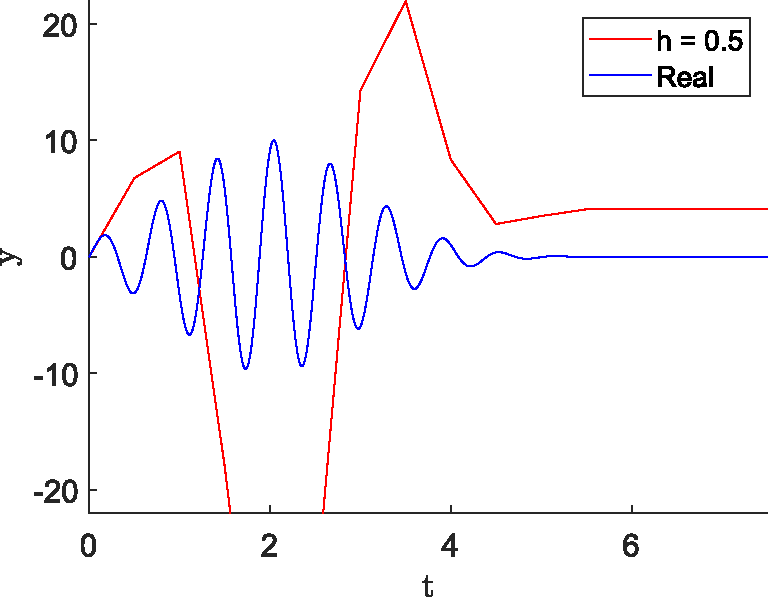
\includegraphics[scale=0.35]{files/rk4vsEuler/euler_05.pdf}}
        \only<2>{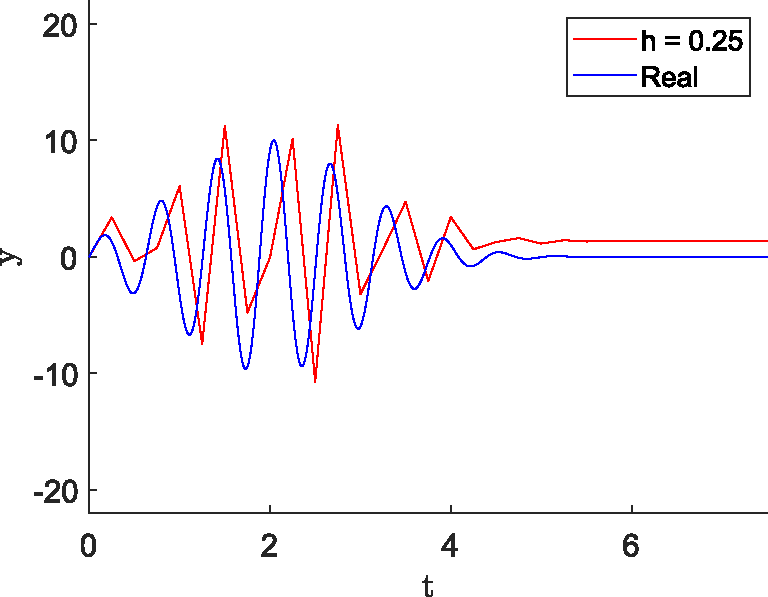
\includegraphics[scale=0.35]{files/rk4vsEuler/euler_025.pdf}}
        \only<3>{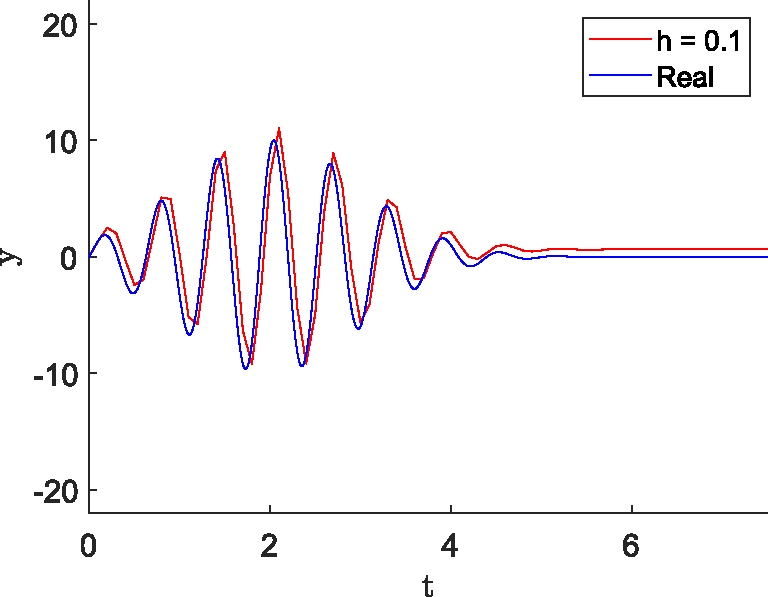
\includegraphics[scale=0.35]{files/rk4vsEuler/euler_01.pdf}}
        \only<4>{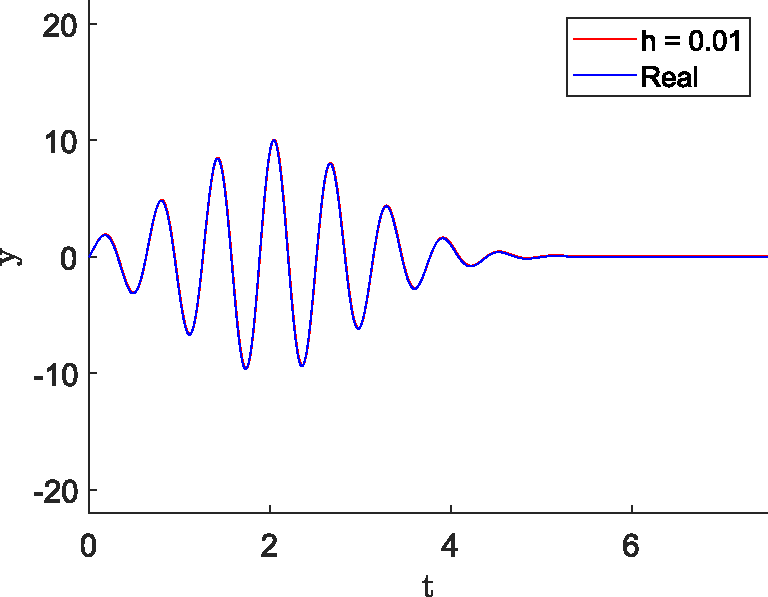
\includegraphics[scale=0.35]{files/rk4vsEuler/euler_001.pdf}}
    \end{figure}\columnbreak$\quad\qquad$\textbf{RK4}
    \vspace{-0.5cm}\begin{figure}[H]
        \centering
        \only<1>{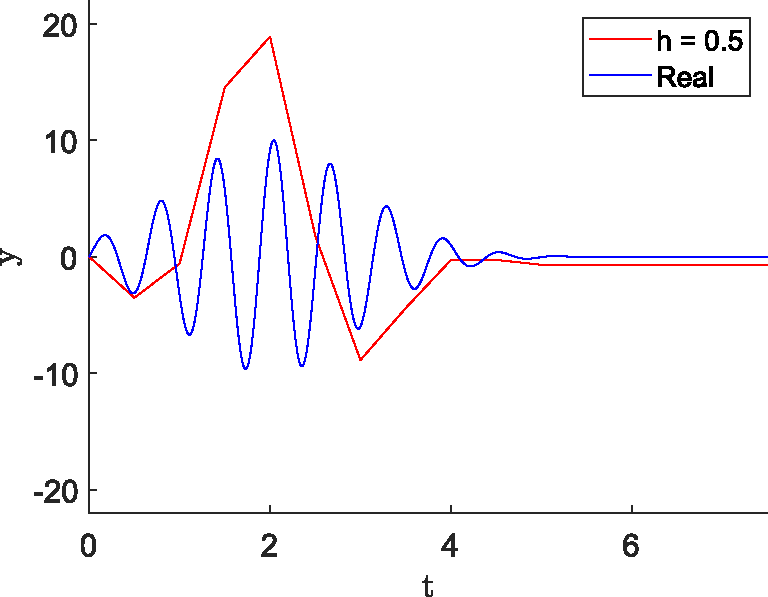
\includegraphics[scale=0.325]{files/rk4vsEuler/rk4_05.pdf}}
        \only<2>{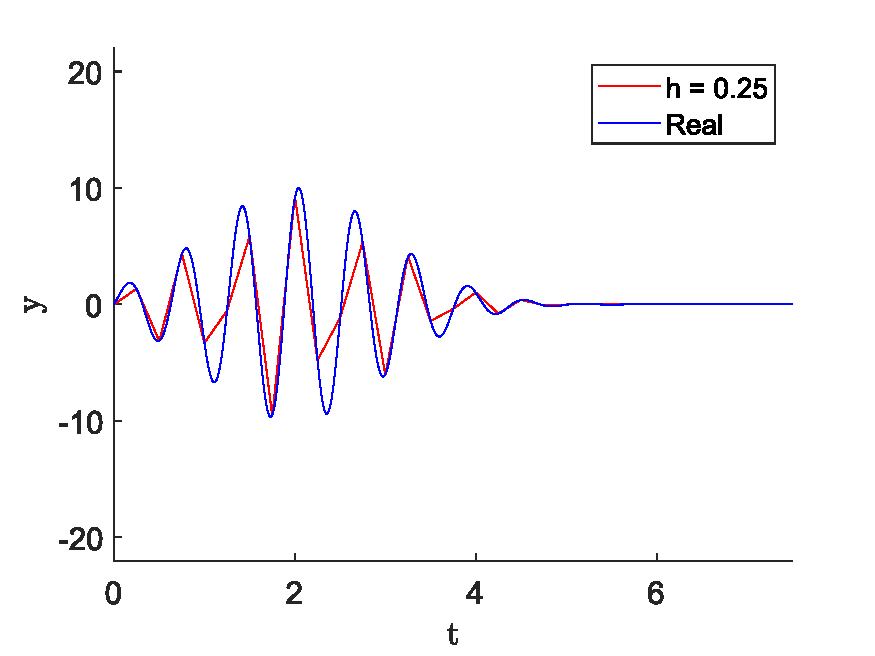
\includegraphics[scale=0.325]{files/rk4vsEuler/rk4_025.pdf}}
        \only<3>{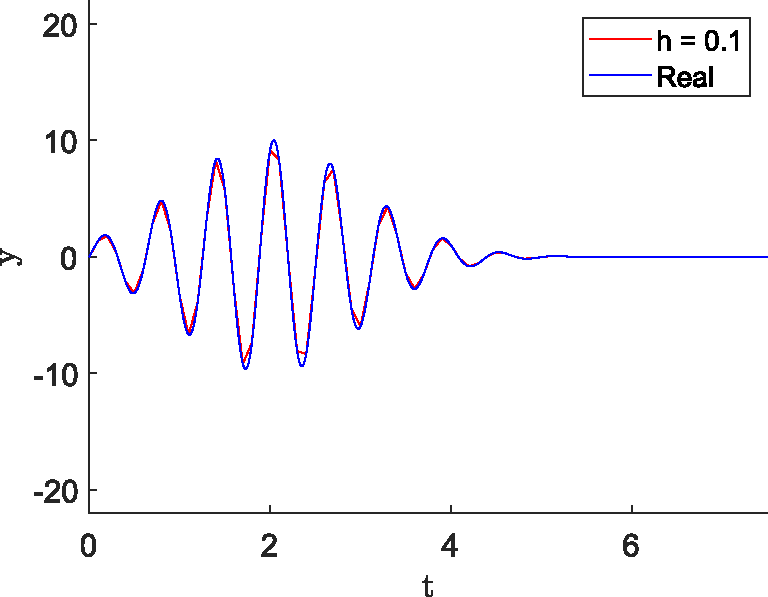
\includegraphics[scale=0.35]{files/rk4vsEuler/rk_01.pdf}}
        \only<4>{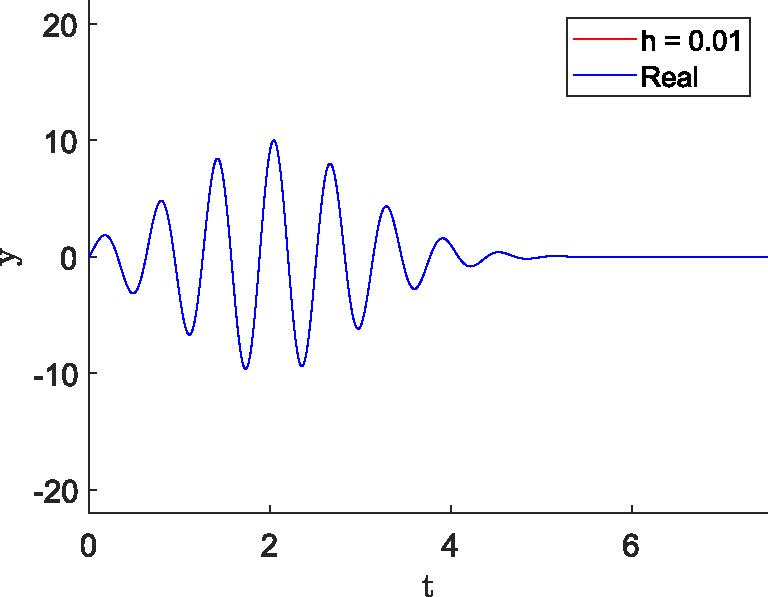
\includegraphics[scale=0.35]{files/rk4vsEuler/rk_001.pdf}}
    
    \end{figure}
\end{multicols}
\end{frame}

\subsection{Systems of ODEs}
\begin{frame}{INTEGER ORDER METHODS}
    \framesubtitle{Systems of ODEs}
    Consider the system of ordinary differential equations
    \begin{equation}
        \begin{cases}
            y_1'=f_1(t,y_1,\,y_2,\,\dots,\,y_n)&y_1(0)=y_{1}\\ y_2'=f_2(t,y_1,\,y_2,\,\dots,\,y_n)&y_2(0)=y_{2}\\
            \qquad\vdots&\\
            y_n'=f_n(t,y_1,\,y_2,\,\dots,\,y_n)&y_n(0)=y_{n}
        \end{cases}
    \end{equation}
    which can be synthesized as 
    \begin{equation}
        \begin{cases}
            \mathbf{y}'=F(t,\mathbf{y})&\\
            \mathbf{y}(0)=\mathbf{y}_0
        \end{cases}
    \end{equation}
    For example, the Lotka-Volterra equations (predator-prey model) is a system of ODEs as follows:
\begin{equation}
    \begin{cases}{y_1'=\alpha y_1-\beta y_1 y_2}& \\ {y_2'=\delta y_1 y_2-\gamma y_2}&\end{cases}
\end{equation}
where $y_1$ represents the number of preys and $y_2$ is the amount of predators.

\end{frame}

\begin{frame}{INTEGER ORDER METHODS}
    \framesubtitle{Systems of ODEs}
\begin{equation}
    \begin{cases}{y_1'=\alpha y_1-\beta y_1 y_2}& \\ {y_2'=\delta y_1 y_2-\gamma y_2}&\end{cases}
\end{equation}
\begin{figure}[H]
    \centering
    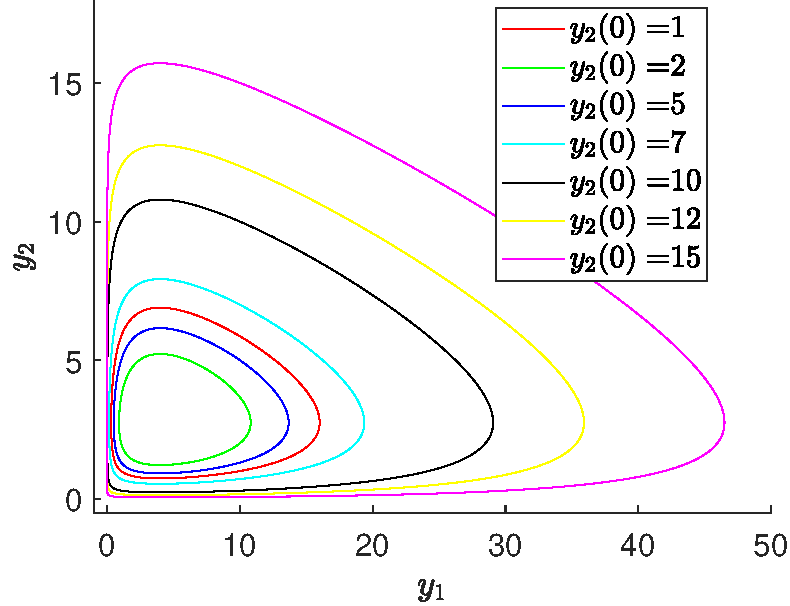
\includegraphics[scale=0.4]{files/Prey.pdf}
    \caption{Phase portrait of Lotka-Volterra equations.}
    \label{fig:lotka}
\end{figure}

\end{frame}

\subsection{Multi-Term ODEs}
\begin{frame}{INTEGER ORDER METHODS}
    \framesubtitle{Multi-Term ODEs}
    In case of higher order ODEs, they can be transformed into a system of first order ODEs, using phase variables $x_i$. Suppose we have an equation as the following:
    \begin{equation}\label{eq:generalDiff}
    \begin{cases}
    y^{(n)}=f\left(t,y,y',...,y^{(n-1)}\right)&\\
    y(0)=y_0,\,\dots,\,y^{(n - 1)}(0)= y_{(n - 1)},\,\,t\in[0,T]&
    \end{cases}
    \end{equation}
    with the following substitution
    \begin{equation}
    \begin{cases}
        x_1 = y&\\
        x_2 = y'&\\
        \qquad\vdots&\\
        x_n = y^{(n-1)}&
    \end{cases}\longrightarrow\begin{cases}
        x_1'=x_2&\\
        x_2'=x_3&\\
        \qquad\vdots&\\
        x_{n-1}'=x_n&\\
        x_n'=f\left(t,x_1,x_2,...,x_{n-1},x_n\right)
    \end{cases}
\end{equation}
\begin{equation*}
    x_1(0)=y_0,\dots,\,x_{n - 1}(0)= y_{(n - 1)}
\end{equation*}

\end{frame}

\begin{frame}{INTEGER ORDER METHODS}
    \framesubtitle{Multi-Term ODEs}
    Example: consider the Duffing oscillator (\href{run:Spring_pendulum.gif}{Click for GIF})
    \begin{equation}
        y''+\delta y'+\alpha y+\beta y^{3}=\gamma \cos (\omega t)
    \end{equation}
    the equivalent system of first order ODEs is
    \begin{equation}
        \begin{cases}
        x_1 = y&\\
        x_2 = y'&\\
    \end{cases}\longrightarrow
    \begin{cases}
        x_1'=x_2&\\
        x_2'=-\delta x_2-\alpha x_1-\beta x_1^3 + \gamma\cos(\omega t)
    \end{cases}
    \end{equation}
    \begin{multicols}{2}
        \begin{figure}[H]
            \centering
            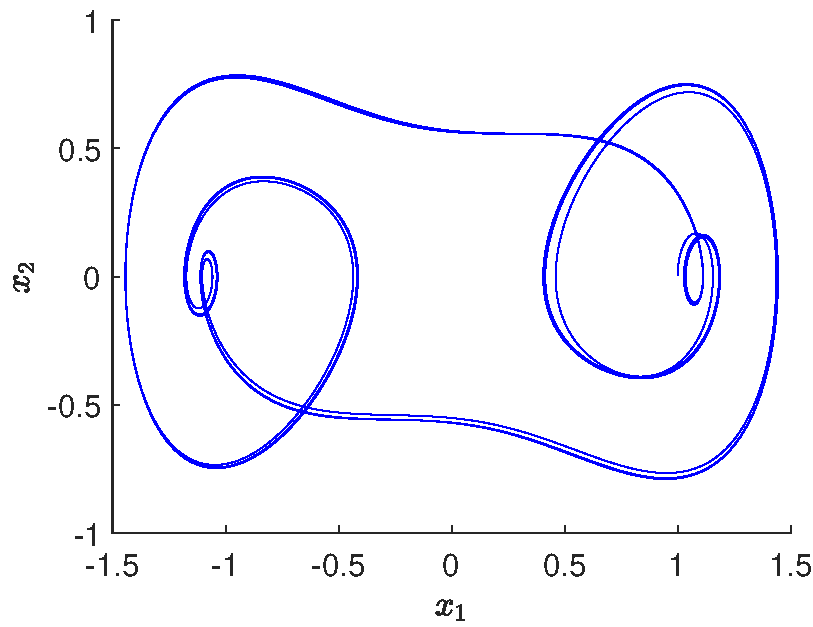
\includegraphics[scale=0.34]{files/Phase.pdf}
        \end{figure}
        \columnbreak
        \begin{figure}[H]
            \centering
            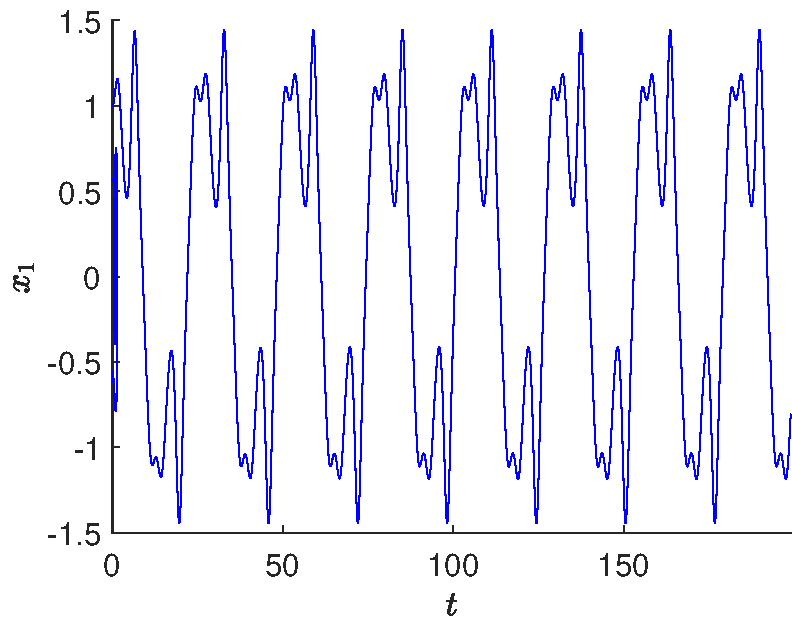
\includegraphics[scale=0.34]{files/Time.pdf}
        \end{figure}
    \end{multicols}
    $\delta=0.3$, $\alpha =-1$, $\beta=1$,$\gamma=0.37$, $\omega =1.2$ and initial conditions $x_1(0)=1$,  $x_2(0)=0$.
\end{frame}


%%%%%%%%%%%% fraccional %%%%%%%%%%

\section{FRACTIONAL ORDER METHODS}
\begin{frame}{FRACTIONAL ORDER METHODS}
Consider the fractional IVP
\begin{equation}\label{eq:frac_dif}
     \begin{cases}
     \dfrac{d^ { \alpha }}{dt^{\alpha }}y(t) = f(t,y)&\\ y(0)=y_0,\,\dots,y^{(m-1)}(0)= y_{(m-1)}\quad \alpha \in \mathbb{R}^+\quad t\in[0,T]&
     \end{cases}
\end{equation}
\begin{multicols}{2}
where $m=\ceil{\alpha}$. \\[0.4cm]\textbf{Example}
\begin{equation}
    \dfrac{d^{0.5}}{dt^{0.5}} y(t)=2\sqrt{\dfrac{y}{\pi}}
\end{equation}
whose solution is \begin{equation}
    y(t)=t
\end{equation}
\columnbreak
\begin{figure}
    \centering
    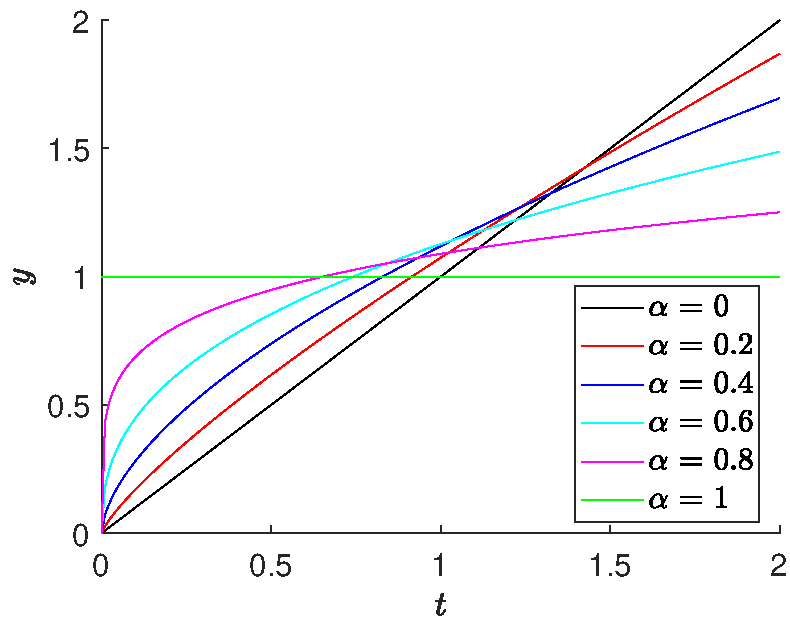
\includegraphics[scale=0.4]{files/t_derivative.pdf}
\end{figure}
\end{multicols}
\end{frame}


\subsection{Adams-Bashforth-Moulton Predictor-Corrector (ABM)}
\begin{frame}{FRACTIONAL ORDER METHODS}
\framesubtitle{Adams-Bashforth-Moulton Predictor-Corrector (ABM)}
Using quadrature theory, the solution can be approximated as
\begin{equation}
    \begin{aligned} y _ { h } \left( t _ { n + 1 } \right) =  \sum _ { k = 0 } ^ { [ \alpha ] - 1 } \frac { t _ { n + 1 } ^ { k } } { k ! } y _ { 0 } ^ { ( k ) } + \frac { h ^ { \alpha } } { \Gamma ( \alpha + 2 ) } f \left( t _ { n + 1 } , y _ { h } ^ { \mathrm { p } } \left( t _ { n + 1 } \right) \right) + \frac { h ^ { \alpha } } { \Gamma ( \alpha + 2 ) } \sum _ { j = 0 } ^ { n } a _ { j , n + 1 } f \left( t _ { j } , y _ { h } \left( t _ { j } \right) \right) \end{aligned}
\end{equation}
\begin{itemize}
    \item $y _ { h } ^ { \mathrm { p } } \left( t _ { n + 1 } \right)$ is a predicted value.
    \item $a _ { j , n + 1 }$ is a quadrature coefficient.
\end{itemize}
The algorithm works as
\begin{center}
    \texttt{y = abm(f,alpha,y0,T,N)}
\end{center}
\begin{itemize}
    \item \texttt{f} is the right-hand side of the differential equation.
    \item \texttt{alpha} is the order of the differential equation.
    \item \texttt{y0} is the initial conditions.
    \item \texttt{T} is the simulation time.
    \item \texttt{N} is the number of partitions on the interval $[0,\text{\texttt{T}}]$.
\end{itemize}
\end{frame}

\begin{frame}{FRACTIONAL ORDER METHODS}
\framesubtitle{Adams-Bashforth-Moulton Predictor-Corrector (ABM)}
\textbf{Example}\\\vspace{0.5cm}
Give an approximate solution to
\begin{equation}
    \begin{cases}
        \dfrac{d^{1.25}}{dt^{1.25}}y(t)=-y(t)&\\
        y'(0)=0,\,y(0)=1
    \end{cases}
\end{equation}

\begin{multicols}{2}
\null \vfill
The exact solution is given by

\begin{equation}
    y(t) = E_{1.25,\,1}(-t^{1.25})=\sum_{k=0}^{\infty}\dfrac{(-1)^kt^{1.25k}}{\Gamma(1.25k +1)}
\end{equation}
\null \vfill
\columnbreak
\begin{figure}[H]
        \centering
        \only<1>{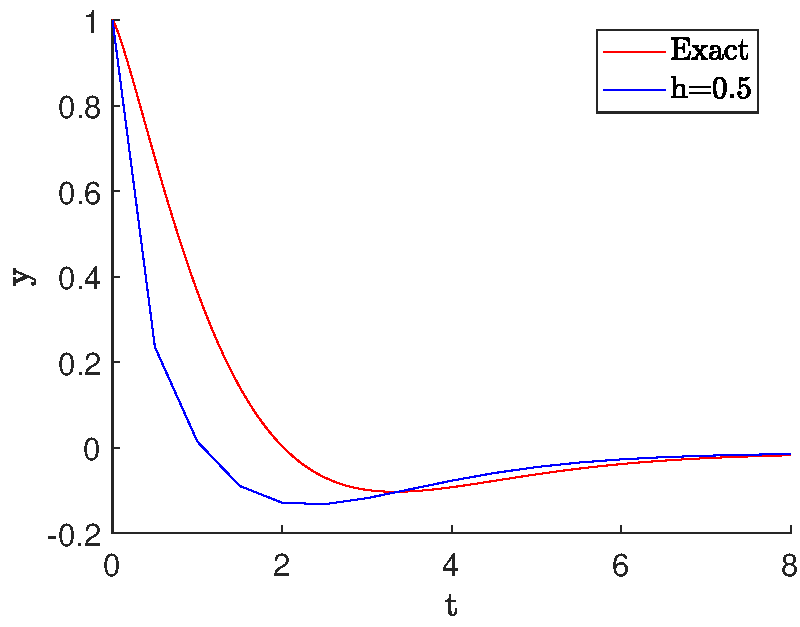
\includegraphics[scale=0.35]{files/comparFrac/ABM_05.pdf}}
        \only<2>{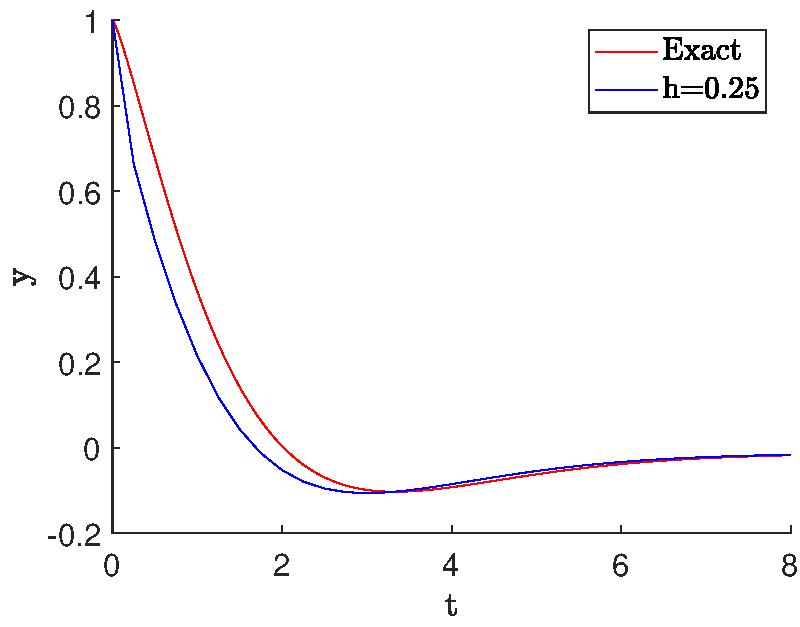
\includegraphics[scale=0.35]{files/comparFrac/ABM_025.pdf}}
        \only<3>{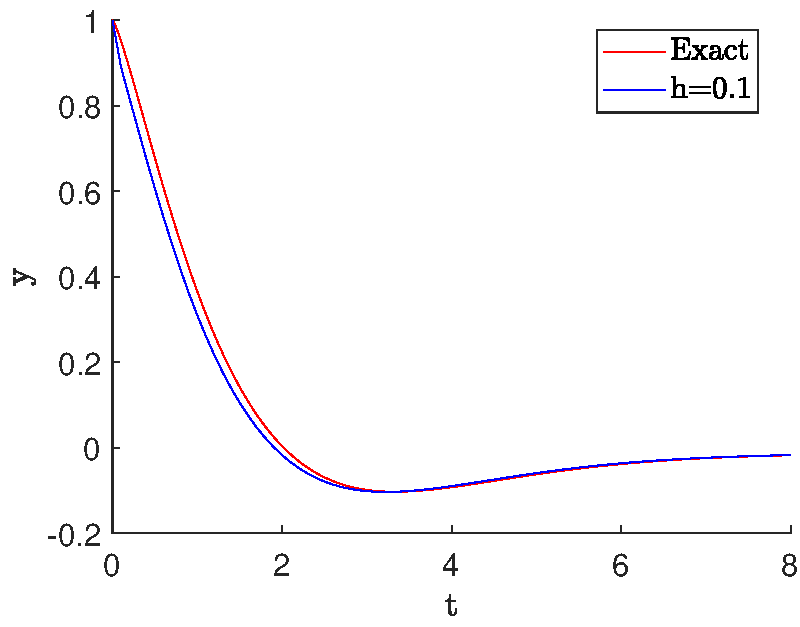
\includegraphics[scale=0.35]{files/comparFrac/ABM_01.pdf}}
        \only<4>{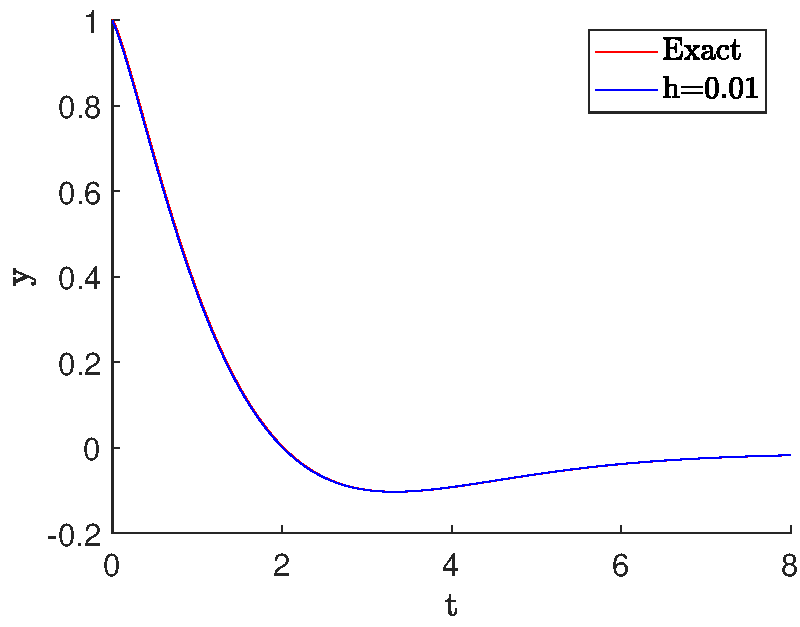
\includegraphics[scale=0.35]{files/comparFrac/ABM_001.pdf}}
    \end{figure}
    \end{multicols}
\end{frame}


\subsection{Decomposition Method}
\begin{frame}{FRACTIONAL ORDER METHODS}
\framesubtitle{Decomposition Method}
Based on decomposing $f$ as follows
    \begin{equation}
        f(t,\mathbf{y})=g(t)+\mathbf{Ay}+h(t,\mathbf{y})
    \end{equation}
Applying the inverse operation to the Caputo fractional derivative
\begin{equation}
    \mathbf{y}(t) = \sum_{r=0}^{m-1}\dfrac{\mathbf{y}_{r}t^r}{r!}+ J^\alpha g(t)+J^\alpha\mathbf{Ay}+J^\alpha h(t,\mathbf{y})
\end{equation}
and supposing a solution in series, we obtain the recursive scheme
\begin{equation}
    \begin{split}
        \mathbf{x}_0&=\sum_{r=0}^{m-1}\dfrac{\mathbf{y}_{r}t^r}{r!}+J^\alpha g(t)\\
        \mathbf{x}_{k+1}&=J^\alpha \mathbf{Ax}_k+J^\alpha \tilde{h}_k\left(t,\sum_{r=0}^k\mathbf{x}_j(t)\right)
    \end{split}
\end{equation}
Where $\tilde{h}_k$ is the Adomian polynomial
\begin{equation}
    \tilde{h}_k\left(t,\sum_{r=0}^{k}\mathbf{x}_j(t)\right)=\dfrac{1}{k!}\left[\dfrac{d^k}{d\lambda^k}h\left(t,\sum_{j=0}^{k}\lambda^j\mathbf{x}_j(t)\right)\Bigg|_{\lambda=0}\right]
\end{equation}
\end{frame}

\begin{frame}{FRACTIONAL ORDER METHODS}
\framesubtitle{Decomposition Method}
The algorithm works as
\begin{center}
    \texttt{ySim = decomposition(f,alpha,y0,N)}
\end{center}
    \textbf{Example}\\\vspace{0.5cm}
Give an approximate solution to
\begin{equation}
    \begin{cases}
        \dfrac{d^{1.25}}{dt^{1.25}}y(t)=-y(t)&\\
        y'(0)=0,\,y(0)=1
    \end{cases}
\end{equation}

\begin{multicols}{2}
\null \vfill
The exact solution is given by

\begin{equation}
    y(t) = E_{1.25,\,1}(-t^{1.25})=\sum_{k=0}^{\infty}\dfrac{(-1)^kt^{1.25k}}{\Gamma(1.25k +1)}
\end{equation}
\null \vfill
\columnbreak
\begin{figure}[H]
        \centering
        \only<1>{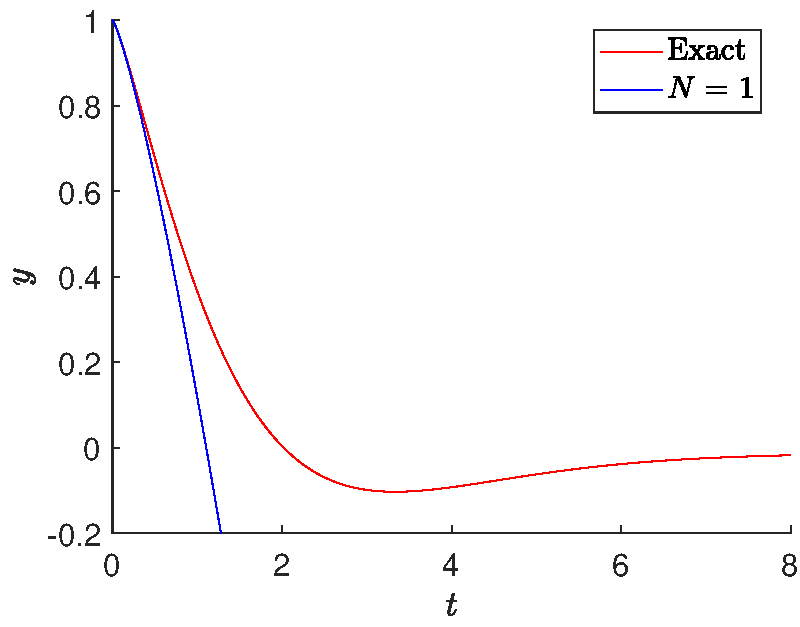
\includegraphics[scale=0.31]{files/comparFrac/Adomian_N_1.pdf}}
        \only<2>{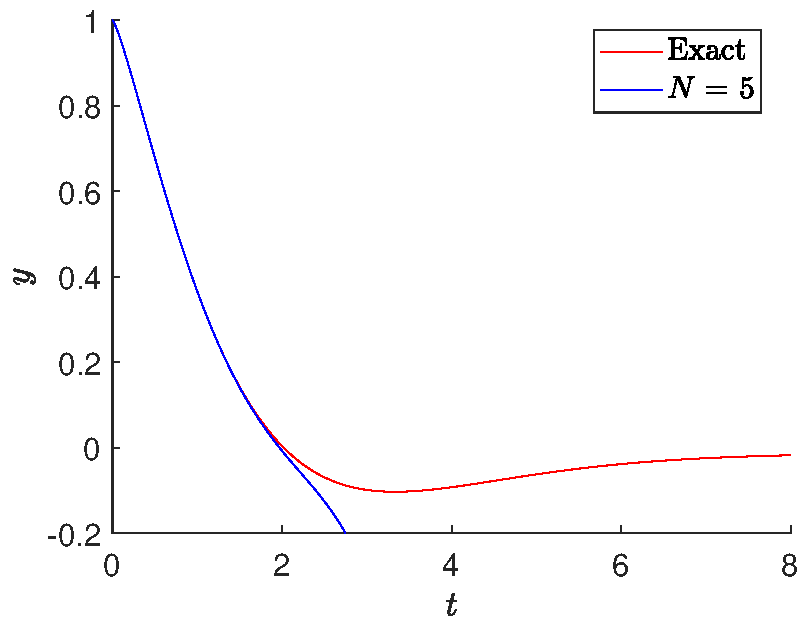
\includegraphics[scale=0.31]{files/comparFrac/Adomian_N_5.pdf}}
        \only<3>{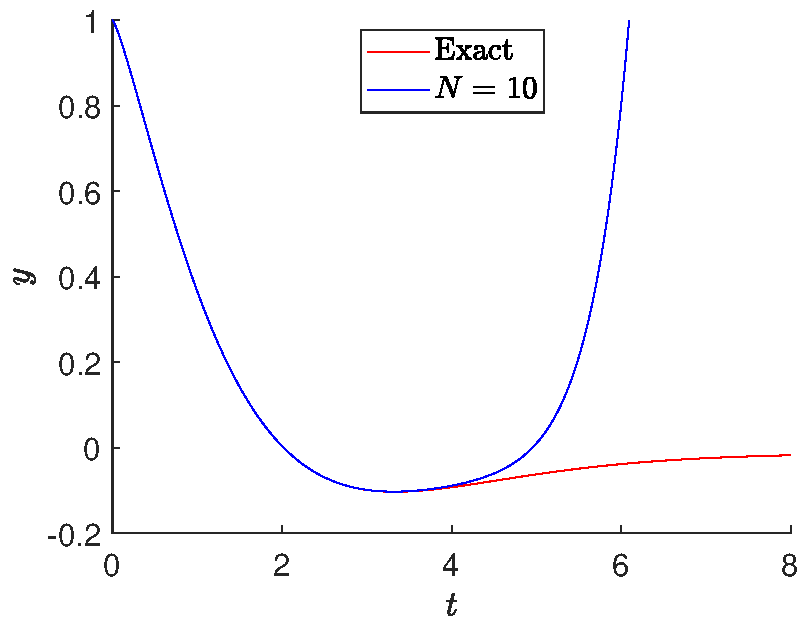
\includegraphics[scale=0.31]{files/comparFrac/Adomian_N_10.pdf}}
        \only<4>{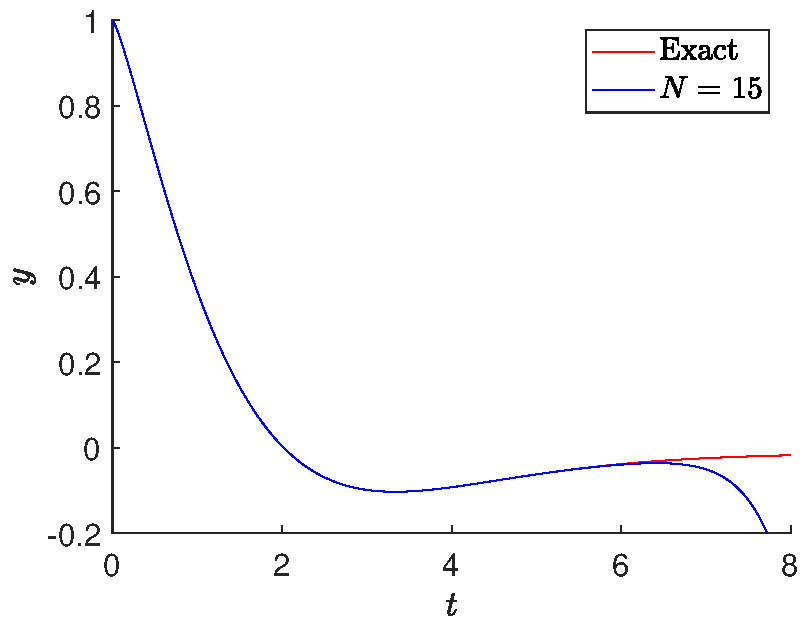
\includegraphics[scale=0.31]{files/comparFrac/Adomian_N_15.pdf}
        }
    \end{figure}
    \end{multicols}
\end{frame}



\subsection{Comparison ABM - Decomposition}
\begin{frame}{FRACTIONAL ORDER METHODS}
\framesubtitle{Comparison ABM - Decomposition}
\begin{equation}
    \begin{cases}
        \dfrac{d^{1.25}}{dt^{1.25}}y(t)=-y(t)&\\
        y'(0)=0,\,y(0)=1
    \end{cases}
\end{equation}

\begin{equation}
    y(t) = E_{1.25,\,1}(-t^{1.25})=\sum_{k=0}^{\infty}\dfrac{(-1)^kt^{1.25k}}{\Gamma(1.25k +1)}
\end{equation}
\begin{multicols}{2}
$\qquad\quad$\textbf{ABM}\begin{figure}[H]
        \centering
        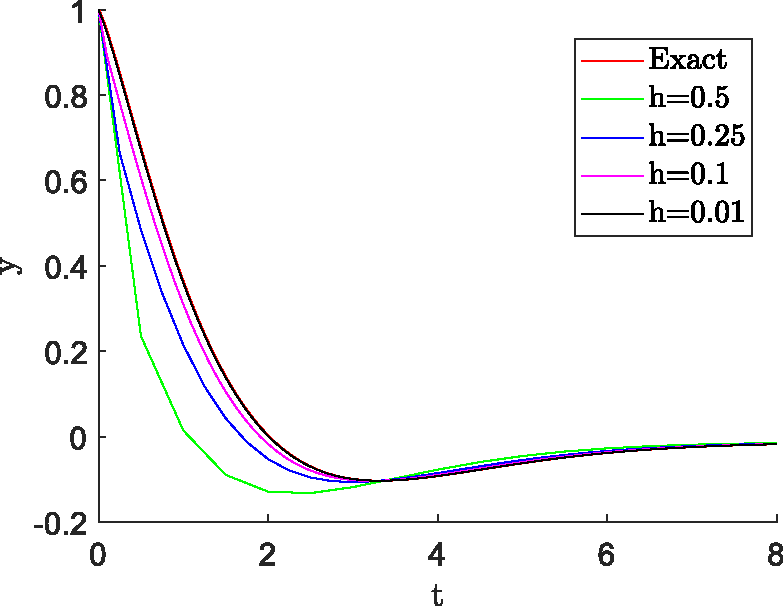
\includegraphics[scale=0.34]{files/ejemplo_adam.pdf}
    \end{figure}\columnbreak$\quad\qquad$\textbf{Decomposition}
    \vspace{-0.5cm}\begin{figure}[H]
        \centering
        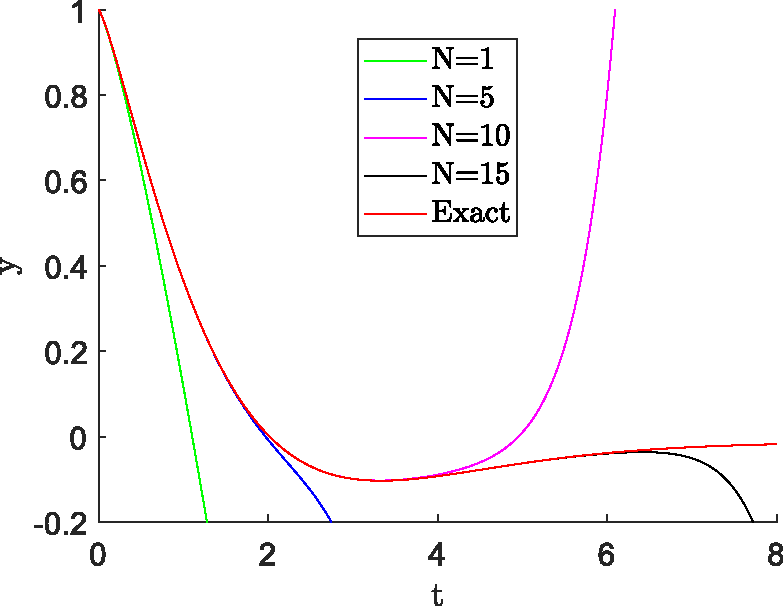
\includegraphics[scale=0.34]{files/frac_deco.pdf}
    \end{figure}
\end{multicols}
\end{frame}

\subsection{Systems of FDEs}
\begin{frame}{FRACTIONAL ORDER METHODS}
    \framesubtitle{Systems of FDEs}
    Consider the system of ordinary fractional differential equations
    \begin{equation}
        \begin{cases}
            \dfrac{d^{\alpha_1}}{dt^{\alpha_1}}y_1=f_1(t,y_1,\,y_2,\,\dots,\,y_n)&y_1(0)=y_{1}\\[6pt] \dfrac{d^{\alpha_2}}{dt^{\alpha_2}}y_2=f_2(t,y_1,\,y_2,\,\dots,\,y_n)&y_2(0)=y_{2}\\
            \qquad\vdots&\\
            \dfrac{d^{\alpha_n}}{dt^{\alpha_n}}y_n=f_n(t,y_1,\,y_2,\,\dots,\,y_n)&y_n(0)=y_{n}\\[6pt]
            \alpha_i\in\mathbb{R}^+,\,\,t\in[0,T]
        \end{cases}
    \end{equation}
    which can be synthesized as 
    \begin{equation}
        \begin{cases}
            \dfrac{d^{\pmb{\alpha}}}{dt^{\pmb{\alpha}}}\mathbf{y}=F(t,\mathbf{y})&\\
            \mathbf{y}(0)=\mathbf{y}_0,\,\pmb{\alpha}\in\left(\mathbb{R}^+\right)^{n\times1},\,t\in[0,T]
        \end{cases}
    \end{equation}
\end{frame}

\subsection{Multi-Term FDEs}
\begin{frame}{FRACTIONAL ORDER METHODS}
\framesubtitle{Multi-Term FDEs}
Suppose we have the multi-term fractional differential equation
\begin{equation}
    \begin{cases}
    \dfrac{d^{\alpha_n}}{dt^{\alpha_n}}y(t)=f\left(t,y,\dfrac{d^{\alpha_{1}}}{dt^{\alpha_{1}}}y,\dfrac{d^{\alpha_{2}}}{dt^{\alpha_{2}}}y,\dots,\dfrac{d^{\alpha_{n-1}}}{dt^{\alpha_{n-1}}}y\right)&\\
    y(0)=y_0,\,\dots,y^{(m-1)}(0)= y_{(m-1)}
    \end{cases}
\end{equation}
    where $m=\ceil{\alpha_n}$ and $0<\alpha_{1}<\alpha_{2}<\ldots<\alpha_{n}$. We select new orders $\tilde{\alpha}_{1}, \ldots, \tilde{\alpha}_{n}$ such that
    \[\begin{array}{l}{\text { (a) } \tilde{\alpha}_{1}, \ldots, \tilde{\alpha}_{n} \text { must be rational numbers, }} \\ {\text { (b) }\left\lceil\alpha_{n}\right\rceil=\left\lceil\tilde{\alpha}_{n}\right\rceil} \\ {\text { (c) } \operatorname{gcd}\left(1, \tilde{\alpha}_{1}, \ldots, \tilde{\alpha}_{n}\right) \text { should be as large as possible, }} \\ {\text { (d) }\left|\alpha_{j}-\tilde{\alpha}_{j}\right| \text { should be as small as possible for all } j}\end{array}\]
\end{frame}


\begin{frame}{FRACTIONAL ORDER METHODS}
\framesubtitle{Multi-Term FDEs}
    We build the approximated system of FDEs with \[\gamma :=\operatorname{gcd}\left(1, \tilde{\alpha}_{1}, \ldots, \tilde{\alpha}_{n}\right)\] 
    \[\tilde{N} :=\frac{\tilde{\alpha}_{n}}{\gamma}\]
    \begin{equation}
    \begin{cases}
    \dfrac{d^{\gamma}}{dt^\gamma} x_{0} =x_{1} &\\[5pt]
    \dfrac{d^{\gamma}}{dt^\gamma} x_{1} =x_{2} &\\
    \qquad\vdots &\\
    \dfrac{d^{\gamma}}{dt^\gamma} x_{\tilde{N}-2} =x_{\tilde{N}-1} &\\[5pt]
    \dfrac{d^{\gamma}}{dt^\gamma} x_{\tilde{N}-1} =f\left(t, x_{0}, x_{\tilde{\alpha}_{1} / \gamma}, \ldots, x_{\tilde{\alpha}_{n-1} / \gamma}\right) \end{cases}
    \end{equation}
    \begin{equation}
    x _ { j } ( 0 ) = \begin{cases} { y _ { ( j \gamma ) }   } & { \text { for } j \gamma \in \mathbb { N } _ { 0 } } \\ { 0  } & { \text { else } } \end{cases}
    \end{equation}
\end{frame}

\begin{frame}{FRACTIONAL ORDER METHODS}
\framesubtitle{Multi-Term FDEs}
    \textbf{Example: Bagley-Torvik Equation} (\href{run:nonNewtonianFluid.gif}{Click for GIF})\\\vspace{0.3cm}
    \begin{equation}
    \begin{cases}
        ay''+b\dfrac{d^{3/2}}{dt^{3/2}}y+cy=g(t)&\\
        y(0)=y_0,\,y'(0)=y_1
    \end{cases}
    \end{equation}
    Let us keep the original orders  $\tilde{\alpha}_1=3/2$ and $\tilde{\alpha}_2=2$ to satisfy condition (d). Note that $\gamma=\operatorname{gcd}(1,3/2,2)=1/2$. Then $\tilde{N}=\dfrac{\tilde{\alpha}_2}{\gamma}=4$. Therefore, the approximated system is
    \begin{equation}
        \begin{cases}
        \dfrac{d^{1/2}}{dt^{1/2}}x_0=x_1&x_0(0)=y_0\\[5pt]
        \dfrac{d^{1/2}}{dt^{1/2}}x_1=x_2&x_1(0)=0\\[5pt]
        \dfrac{d^{1/2}}{dt^{1/2}}x_2=x_3&x_2(0)=y_1\\[5pt]
        \dfrac{d^{1/2}}{dt^{1/2}}x_3=f\left(t,x_0,x_{1.5/0.5}\right)=\dfrac{g(t)-cx_0-bx_3}{a}&x_3(0)=0\\
        \end{cases}
    \end{equation}
\end{frame}

\begin{frame}{FRACTIONAL ORDER METHODS}
\framesubtitle{Multi-Term FDEs}
    \textbf{Example: Bagley-Torvik Equation}\\\vspace{0.5cm}
    In particular, for $a=1$, $b=c=-1$, $g(t)=t+1$, $y_0=1$ and $y_1=1$, the exact solution to this IVP is 
    \begin{equation}
        y(t)=1+t
    \end{equation}
    \begin{figure}[H]
        \centering
        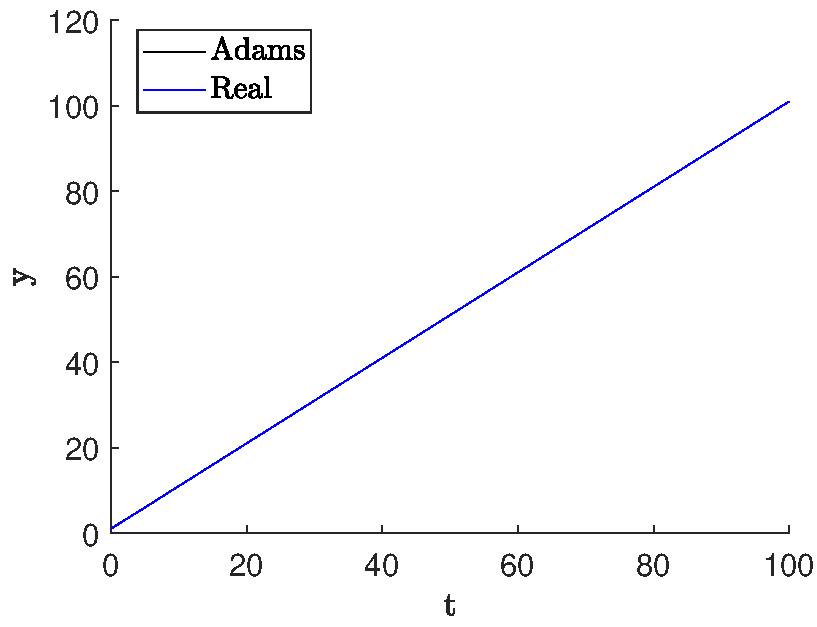
\includegraphics[scale=0.45]{files/abm_system.pdf}
    \end{figure}
\end{frame}





